%%%%%%%%%%%%%%%%%%%%%%%%%%%%%%%%%%%%%%%%%
% Thesis 
% LaTeX Template
% Version 1.3 (21/12/12)
%
% This template has been downloaded from:
% http://www.latextemplates.com
%
% Original authors:
% Steven Gunn 
% http://users.ecs.soton.ac.uk/srg/softwaretools/document/templates/
% and
% Sunil Patel
% http://www.sunilpatel.co.uk/thesis-template/
%
% License:
% CC BY-NC-SA 3.0 (http://creativecommons.org/licenses/by-nc-sa/3.0/)
%
% Note:
% Make sure to edit document variables in the Thesis.cls file
%
%%%%%%%%%%%%%%%%%%%%%%%%%%%%%%%%%%%%%%%%%

%----------------------------------------------------------------------------------------
%	PACKAGES AND OTHER DOCUMENT CONFIGURATIONS
%----------------------------------------------------------------------------------------


\documentclass[11pt, a4paper, oneside]{Thesis} % Paper size, default font size and one-sided paper

\graphicspath{{./Pictures/}} % Specifies the directory where pictures are stored

\usepackage[utf8]{inputenc}
\usepackage[square, numbers, comma, sort&compress]{natbib} % Use the natbib reference package - read up on this to edit the reference style; if you want text (e.g. Smith et al., 2012) for the in-text references (instead of numbers), remove 'numbers' 
\hypersetup{urlcolor=blue, colorlinks=true} % Colors hyperlinks in blue - change to black if annoying
\title{\ttitle} % Defines the thesis title - don't touch this

\begin{document}

\frontmatter% Use roman page numbering style (i, ii, iii, iv...) for the pre-content pages

\setstretch{1.3} % Line spacing of 1.3

% Define the page headers using the FancyHdr package and set up for one-sided printing
\fancyhead{} % Clears all page headers and footers
\rhead{\thepage} % Sets the right side header to show the page number
\lhead{} % Clears the left side page header

\pagestyle{fancy} % Finally, use the "fancy" page style to implement the FancyHdr headers

\newcommand{\HRule}{\rule{\linewidth}{0.5mm}} % New command to make the lines in the title page

% PDF meta-data
\hypersetup{pdftitle={\ttitle}}
\hypersetup{pdfsubject=\subjectname}
\hypersetup{pdfauthor=\authornames}
\hypersetup{pdfkeywords=\keywordnames}

%----------------------------------------------------------------------------------------
%	TITLE PAGE
%----------------------------------------------------------------------------------------

\begin{titlepage}
\begin{center}

\textsc{\LARGE \univname}\\[1.5cm] % University name
\textsc{\Large Master Thesis}\\[0.5cm] % Thesis type

\HRule \\[0.4cm] % Horizontal line
{\huge \bfseries \ttitle}\\[0.4cm] % Thesis title
\HRule \\[1.5cm] % Horizontal line
 
\begin{minipage}{0.4\textwidth}
\begin{flushleft} \large
\emph{Author:}\\
{\authornames} % Author name - remove the \href bracket to remove the link
\end{flushleft}
\end{minipage}
\begin{minipage}{0.4\textwidth}
\begin{flushright} \large
\emph{Supervisor:} \\
{\supname} % Supervisor name - remove the \href bracket to remove the link  
\end{flushright}
\end{minipage}\\[3cm]
 
\large \textit{A thesis submitted in fulfilment of the requirements\\ for the degree of \degreename}\\[0.3cm] % University requirement text
\textit{in the}\\[0.4cm]
\groupname\\\deptname\\[2cm] % Research group name and department name
 
{\large \today}\\[4cm] % Date
%\includegraphics{Logo} % University/department logo - uncomment to place it
 
\vfill
\end{center}

\end{titlepage}

%----------------------------------------------------------------------------------------
%	DECLARATION PAGE
%	Your institution may give you a different text to place here
%----------------------------------------------------------------------------------------

\Declaration{

\addtocontents{toc}{\vspace{1em}} % Add a gap in the Contents, for aesthetics

I, \authornames, declare that this thesis titled, '\ttitle' and the work presented in it are my own. I confirm that:

\begin{itemize} 
\item[\tiny{$\blacksquare$}] This work was done wholly or mainly while in candidature for a research degree at this University.
\item[\tiny{$\blacksquare$}] Where any part of this thesis has previously been submitted for a degree or any other qualification at this University or any other institution, this has been clearly stated.
\item[\tiny{$\blacksquare$}] Where I have consulted the published work of others, this is always clearly attributed.
\item[\tiny{$\blacksquare$}] Where I have quoted from the work of others, the source is always given. With the exception of such quotations, this thesis is entirely my own work.
\item[\tiny{$\blacksquare$}] I have acknowledged all main sources of help.
\item[\tiny{$\blacksquare$}] Where the thesis is based on work done by myself jointly with others, I have made clear exactly what was done by others and what I have contributed myself.\\
\end{itemize}
 
Signed:\\
\rule[1em]{25em}{0.5pt} % This prints a line for the signature
 
Date:\\
\rule[1em]{25em}{0.5pt} % This prints a line to write the date
}

\clearpage % Start a new page

%----------------------------------------------------------------------------------------
%	QUOTATION PAGE
%----------------------------------------------------------------------------------------

%\pagestyle{empty} % No headers or footers for the following pages

%\null\vfill % Add some space to move the quote down the page a bit

%\textit{``Thanks to my solid academic training, today I can write hundreds of words on virtually any topic without possessing a shred of information, which is how I got a good job in journalism."}

%\begin{flushright}
%Dave Barry
%\end{flushright}

%\vfill\vfill\vfill\vfill\vfill\vfill\null % Add some space at the bottom to position the quote just right

%\clearpage % Start a new page

%----------------------------------------------------------------------------------------
%	ABSTRACT PAGE
%----------------------------------------------------------------------------------------

\addtotoc{Abstract} % Add the "Abstract" page entry to the Contents

\abstract{\addtocontents{toc}{\vspace{1em}} % Add a gap in the Contents, for aesthetics

The Thesis Abstract is written here (and usually kept to just this page). The page is kept centered vertically so can expand into the blank space above the title too\ldots
}

\clearpage % Start a new page

%----------------------------------------------------------------------------------------
%	ACKNOWLEDGEMENTS
%----------------------------------------------------------------------------------------

\setstretch{1.3} % Reset the line-spacing to 1.3 for body text (if it has changed)

\acknowledgements{\addtocontents{toc}{\vspace{1em}} % Add a gap in the Contents, for aesthetics

The acknowledgements and the people to thank go here, don't forget to include your project advisor\ldots
}
\clearpage % Start a new page

%----------------------------------------------------------------------------------------
%	LIST OF CONTENTS/FIGURES/TABLES PAGES
%----------------------------------------------------------------------------------------

\pagestyle{fancy} % The page style headers have been "empty" all this time, now use the "fancy" headers as defined before to bring them back

\lhead{\emph{Contents}} % Set the left side page header to "Contents"
\tableofcontents % Write out the Table of Contents

\lhead{\emph{List of Figures}} % Set the left side page header to "List of Figures"
\listoffigures % Write out the List of Figures

\lhead{\emph{List of Tables}} % Set the left side page header to "List of Tables"
\listoftables % Write out the List of Tables

%----------------------------------------------------------------------------------------
%	ABBREVIATIONS
%----------------------------------------------------------------------------------------

\clearpage % Start a new page

\setstretch{1.5} % Set the line spacing to 1.5, this makes the following tables easier to read

\lhead{\emph{Abbreviations}} % Set the left side page header to "Abbreviations"
\listofsymbols{ll} % Include a list of Abbreviations (a table of two columns)
{
\textbf{LAH} & \textbf{L}ist \textbf{A}bbreviations \textbf{H}ere \\
%\textbf{Acronym} & \textbf{W}hat (it) \textbf{S}tands \textbf{F}or \\
}

%----------------------------------------------------------------------------------------
%	PHYSICAL CONSTANTS/OTHER DEFINITIONS
%----------------------------------------------------------------------------------------

%\clearpage % Start a new page

%\lhead{\emph{Physical Constants}} % Set the left side page header to "Physical Constants"

%\listofconstants{lrcl} % Include a list of Physical Constants (a four column table)
%{
%Speed of Light & $c$ & $=$ & $2.997\ 924\ 58\times10^{8}\ \mbox{ms}^{-\mbox{s}}$ (exact)\\
% Constant Name & Symbol & = & Constant Value (with units) \\
%}

%----------------------------------------------------------------------------------------
%	SYMBOLS
%----------------------------------------------------------------------------------------

%\clearpage % Start a new page

%\lhead{\emph{Symbols}} % Set the left side page header to "Symbols"

%\listofnomenclature{lll} % Include a list of Symbols (a three column table)
%{
%$a$ & distance & m \\
%$P$ & power & W (Js$^{-1}$) \\
% Symbol & Name & Unit \\

%& & \\ % Gap to separate the Roman symbols from the Greek

%$\omega$ & angular frequency & rads$^{-1}$ \\
% Symbol & Name & Unit \\
%}

%----------------------------------------------------------------------------------------
%	DEDICATION
%----------------------------------------------------------------------------------------

%\setstretch{1.3} % Return the line spacing back to 1.3

%\pagestyle{empty} % Page style needs to be empty for this page

%\dedicatory{For/Dedicated to/To my\ldots} % Dedication text

%\addtocontents{toc}{\vspace{2em}} % Add a gap in the Contents, for aesthetics

%----------------------------------------------------------------------------------------
%	THESIS CONTENT - CHAPTERS
%----------------------------------------------------------------------------------------

\mainmatter % Begin numeric (1,2,3...) page numbering

\pagestyle{fancy} % Return the page headers back to the "fancy" style

% Include the chapters of the thesis as separate files from the Chapters folder
% Uncomment the lines as you write the chapters

% Chapter Template

\chapter{Introduction} % Main chapter title

\label{Chapter1} % Change X to a consecutive number; for referencing this chapter elsewhere, use \ref{ChapterX}

\lhead{Chapter 1. \emph{Introduction}} % Change X to a consecutive number; this is for the header on each page - perhaps a shortened title

These days, information is very important. Not only information itself, but the \emph{access} to it is paramount. Most information is found there, where everyone contributes to - the world wide web. Here we have many contributors (authors, engineers, teachers, ...) on many different sites and this means: fragmented information. Even if a certain piece of information is there we can't \emph{access} it, because we don't know where to find it. That's unsatisfying and that's why search engines \footnote{\url{http://en.wikipedia.org/wiki/Web_search_engine}} are so important to us.
\newline
Unfortunately, today, only a few big companies are able to deal with both the engineering challenge and the resource requirements needed to operate a good search engine. They collect all the information and give us \emph{access} to it. What's even more frustrating is that we don't really know \emph{how} they do it. In order to better understand, research is ongoing in diverse domains of search engines.
\newline
A lot of work has been done in page importance algorithms (selection policies) or what pages need to be crawled how often (re-visit policies)\cite{page_importance1}\cite{page_importance2}. At the end, assuming that we selected the optimal set of pages, we need to be able to download them in parallel and efficiently (parallelisation policy). This is where crawl.js wants to contribute. Building a high performance crawling architecture capable of downloading thousands of pages per second is a rather practical problem and relatively few work has been done on this specific topic \cite{ubicrawler}\cite{hp_crawler}. Additionally, at the time of writing, there is no crawling architecture that is distributed and locality-aware\footnote{Crawlers should fetch pages near them (in terms of latency)} that we know of.

\section{Node.js \& Redis}
We built Crawl.js using the JavaScript environment Node.js\footnote{\url{http://www.nodejs.org}}. As quoted: "Node.js uses an event-driven, non-blocking I/O model that makes it lightweight and efficient, perfect for data-intensive real-time applications that run across distributed devices." Regarding that a web crawler is data driven and resource intensive, using such an environment seemed a good choice. Additionally there is no other web crawler that we know of running on Node.js and making intensive use of redis\footnote{\url{http://redis.io}} to manage URLs.

\section{Outline}
In Chapter~\ref{Chapter2} we summarize the related work in the research domain of our thesis. Afterwards, we discuss more in detail the specific problems we want to contribute to in Chapter~\ref{Chapter3}. The Chapters ~\ref{Chapter4} and ~\ref{Chapter5} give insights how Crawl.js works and how it performs during our experiments. Finally, we come to some conclusions in Chapter~\ref{Chapter6} and mention some ideas for the future of Crawl.js.

\chapter{Related work} % Main chapter title
The research area of web crawling in general is large. In this thesis, we want to focus on the work that has been done regarding architectures of web crawlers. Only a few have actually tried to build a scalable, parallel and distributed web crawler. In the following, the sections present related works sorted by themes.
\label{Chapter2} % Change X to a consecutive number; for referencing this chapter elsewhere, use \ref{ChapterX}
\lhead{Chapter 2. \emph{Related work}} % Change X to a consecutive number; this is for the header on each page - perhaps a shortened title

\section{Sequential crawlers}
One page is downloaded at the time. Nothing happens in parallel. Theses kind of web crawlers were used in the very beginning of the web. As the number of web pages grew the need to download web pages at a higher rate was obvious.

\section{Parallel centralized crawlers}
This kind of crawlers use several distinct components in their system. Each component is typically responsible for one or more specific tasks (ex. Downloader, Manager, Resolver). There is always one component that takes the role of a manager and is therefore \emph{central}. Such systems are more difficult to scale.

\subsection{Design and Implementation of a High-Performance Distributed Web Crawler~\cite{hp_crawler}}
This crawler design is separated into two main components, referred to as \emph{crawling application} and \emph{crawling system}. The crawling application decides which URLs to download next (ex. Breadth-first, focused), whereas the crawling system is responsible for handling the stream of URLs efficiently. Figure~\ref{hp_crawler} shows an overview of the system.
\begin{figure}[h]
\centering
  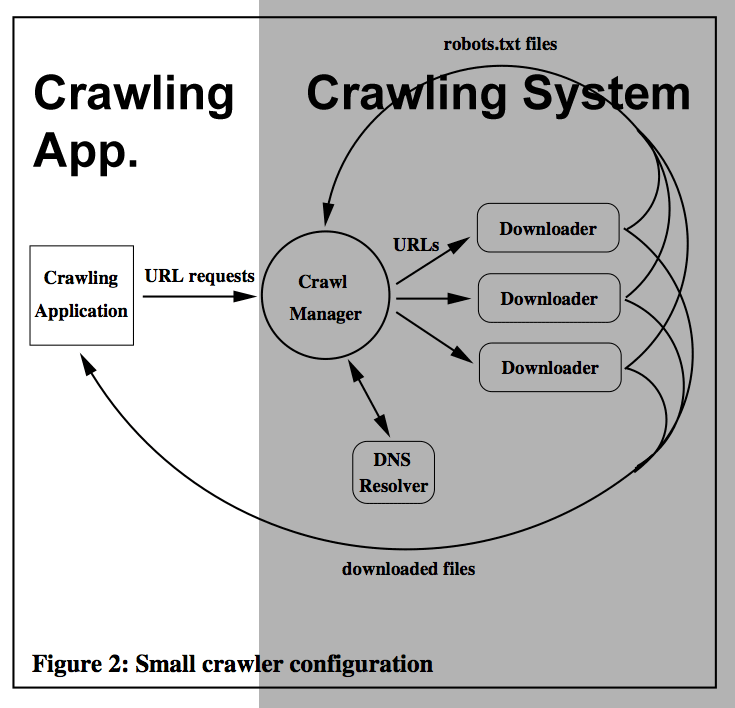
\includegraphics[width=0.7\textwidth]{Figures/hp_crawler.png}
\caption{System Architecture centralized crawler (High-Performance Distributed Web Crawler)}
\label{hp_crawler}
\end{figure}
As you can see `The crawl manager is the central component of the system'. Following the path of an URL (starting from the Crawl Manager) leads us to the \emph{Downloader} and back to the Crawling application. Scaling such a system is possible but requires more effort than in decentralized systems. How a larger system might look like is described in detail but we will not discuss it further because of other architectural design choices of Crawl.js.
Interestingly, the details discussed in section \emph{Implementation Details and Algorithmic Techniques} revealed common problems and were of great use for Crawl.js:
\begin{itemize}
  \item Parsing using regular expressions\footnote{\url{http://en.wikipedia.org/wiki/Regular_expression}} will be evaluated against regular parsing.
  \item The insight `We first note that fetching URLs in the order they were parsed out of the pages is a very bad idea, since there is a lot of second-level domain locality in the links' will be respected during the implementation phase of Crawl.js.
\end{itemize}


\section{Parallel decentralized crawlers}
Decentralized crawlers do not have a central managing unit. Typically those systems have identifiable and equal workers which are responsible for a certain piece of work. Such a system is fully distributed and easily scalable (increase in the number of workers). Of course there is some sort of communication between the workers, but the important point is that each worker is equal and autonomic.

\subsection{UbiCrawler: a scalable fully distributed Web crawler \cite{ubicrawler}}
UbiCrawler have multiple identically implemented workers (called agents). Every worker has an identity and is responsible for a defined set of URLs. For a given URL every worker is able to compute the identity responsible for that URL locally. This reduces the intercommunication overhead between the different workers in the system. The component used to compute a workers identity (based on a URL) is called \emph{assignment function}. It is important to note here, that the function directly assigns an identity of a worker. To be more precise, a worker that is alive and healthy. This fact of direct assignment leads to a problem UbiCrawler needs to solve. What happens if the assigned worker crashes? In this case it must be guaranteed that the function reassigns the same worker after he is back alive. (For a rapidly changing total set of URLs). So they need an assignment function that is:
\begin{itemize}
\item Random, to properly load balance the system,
\item Local, to deal with the problem of joining/leaving workers,
\item Contravariant, adding new workers, shrinks the workload (set of URLs) of one worker.
\end{itemize}
Satisfying two of those requirements Random and Contravariant is easily achievable with a simple modulo function on the hash of the URL for example. The information every worker must know at anytime is the total number of workers in the system. Satisfying the third one is more complex and they solved it using a modified version of \emph{consistent hashing} called \emph{Identifier–Seeded Consistent Hashing}. 

Crawl.js will try to circumvent this complexity by adding an additional layer between the assignment function and the responsible worker. In Crawl.js, the assignment function doesn't assign an identity of a worker but an identity of a bucket. A bucket is nothing more than a persistent queue. So the assignment function doesn't know anything about workers. In a second step, Crawl.js will assign workers to those buckets. Using this additional layer removes complexity to the assignment function while keeping fault tolerance capabilities. This is achieved by flagging processed URLs within the bucket.
 
% Chapter Template
\chapter{Problem description} % Main chapter title
Building a slow crawler that runs on one machine and downloads several pages per minute is easy. Designing and implementing a distributed and parallel web crawler presents a number of challenges. In this chapter we want to discuss those more in detail.

\label{Chapter3} % Change X to a consecutive number; for referencing this chapter elsewhere, use \ref{ChapterX}

\lhead{Chapter 3. \emph{Problem description}} % Change X to a consecutive number; this is for the header on each page - perhaps a shortened title

\section{Size of the web}
Today (Thursday, 09 May, 2013) the size of the world wide web is at least 14.78 billion (10\textsuperscript{9}) indexed pages.\cite{wwwsize}

Here is a simple calculation to demonstrate how long it takes to download the entire web if you fetch one page after the other.
Lets assume an average page size of \textbf{320KB} \cite{webmetrics} (including resources such as images, scripts and stylesheets) and an ideal network connection of \textbf{100mbit/s}.

Based on these numbers it would take \textbf{~11.7 years}. And it becomes worse when you add a realistic latency of 100msec per page which adds another \textbf{~47 years} of idle time. So, in total it takes \textbf{58.7 years}.

As you see, if we want to download the web in a reasonable amount of time we have to \textbf{split} and \textbf{distribute} the work so that we can work in \textbf{parallel}.

\section{Parallel work}
Lets discuss the challenges in splitting and distributing the work.
\subsection{Split}
How do we split the huge amount of work equally? We need pieces of work that we can distribute to different workers. The pieces should be:
\begin{itemize}
\item Mutual exclusive (we dont want to download pages twice)
\item Equally sized.
\item Clustered in terms of \textbf{closeness}.
\end{itemize}
Additionally we have another challenge. The total amount of work is growing and therefore we need to be able to adjust the splitting dynamically. If one piece becomes too big we need to be able to split it further.
\subsection{Distribute}
Once we have splitted the work we can distribute the smaller work pieces to different workers. This has to be done in such a way that every piece of work is assigned to one worker only. Additionally we want that the work load of all workers is more or less the same. This leads us to another problem we have to work on: \textbf{Load-balancing}.
\subsection{Load-balance}
What worker should work on which work piece next? so that:
\begin{itemize}
\item Every worker is busy.
\item No worker is idleing.
\item The worker is working on a piece best suited for him. (\textbf{Performance})
\end{itemize}
The balancer should recognise workers taking too long to do one piece of work and be able take appropriate actions.

\section{Performance}
The reason why we \textbf{split} and \textbf{distribute} the work is performance. We want to minimize the time to download all pages. Doing it in parallel is not sufficient, we need to tackle a lot more challenges. The number of optimizations one could think of is probably infinite. Here are the major challenges we want to solve.
\subsection{Closeness}
\label{closeness}
In order to optimize a particular worker, the worker should be \textbf{close} in terms of:
\begin{itemize}
\item Latency
\item Geo Location
\end{itemize}
\subsection{Decentralized}
We don't want a \textbf{central} bottleneck unit. Every component in the system should be intelligent and able to decide what to do next on his own.


\chapter{Crawl.js} % Main chapter title
In this chapter we describe how crawl.js splits and distributes the work in detail.
\label{Chapter4} 
\lhead{Chapter 4. \emph{Crawl.js}} 

\section{System overview}
Crawl.js is a decentralized system. Each \emph{worker} in the system is standalone and autonomous and does not depend on any other worker. The only thing a worker needs is a connection to the \emph{Queues} and the \emph{Stores}. Figure~\ref{system_overview} gives an overview of the main components in the system.

Lets follow the path of an URL in the system.
The first thing a worker needs to do is get some URLs (1) from a remote queue (Note that the worker knows by his own which Queue to ask). Step 2 and 3 involves fetching, parsing and storing the content given by the URL. Thanks to the asynchronous nature (Streaming) of Crawl.js the parsing (3) can happen before the fetching (2) is done. Even storing the content (3) is done while fetching. More on this later. Whenever a new URL is extracted in the parsing step it is added to the \emph{Queue}. The queue then decides what to do (\emph{4a},\emph{4b}). Either it is kept in the local (in-memory) queue or dispatched to a remote one (batch processing).

\begin{figure}[h]
\centering
  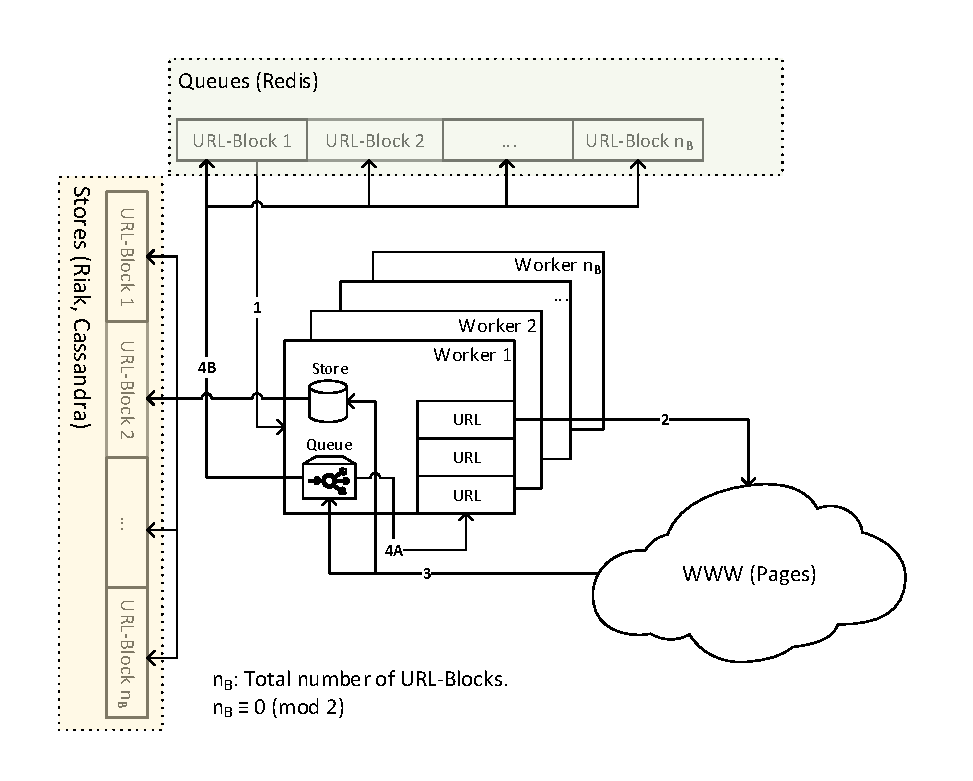
\includegraphics[width=1\textwidth]{Figures/system_overview.pdf}
\caption{Crawl.js - System Overview}
\label{system_overview}
\end{figure}

\section{Mapper}
\label{mapper}
The mapper is not a physical component in the system like the \emph{Queue}, the \emph{Worker} or the \emph{Store}. It is a algorithm allowing each component at any time to map an URL to an identifier. This identifier is then primarily used to determine the responsible \emph{Queue} or \emph{Store} for that URL.
This ability of being able to compute an identifier for a URL \emph{independently} is key to the whole system architecture. This ability is what makes the system decentralized. We don't have to ask a central component with manager like capabilities. We can compute the identifier ourself. Basically it identifies a virtual block within the URL space (all URLs). Every URL belongs to one and only one virtual block and each block is:
\begin{itemize}
  \item Mutual exclusive - Each block belongs to one and one worker only.
  \item Equally sized - From block to block the number of URLs should roughly be the same.
\end{itemize}

In other words the mapper is responsible to \emph{split} the work. In Crawl.js the mapper is nothing more than a function implemented as a separate module. Each component that needs to be able to map an URL to an identifier just include the module. The algorithm used is rather simple and illustrated below:
\begin{algorithmic}[0]
\Function{Map}{$url$}\Comment{Map the URL to an identifier}
\State $host \gets url.host$\Comment{Only the host part ex. www.unine.ch}
\State $hash \gets \textbf{hash}(host)$\Comment{Hash the host part}
\State $id \gets hash \bmod n$\Comment{id $\in \{0,1,..n\}$, n:total number of virtual blocks}
\State \textbf{return} $id$
\EndFunction
\end{algorithmic}

So the idea is to hash the host part of the URL modulo the total number of blocks we want. The modulo number (total number of blocks) must be shared among every component using the mapper in the system.
To achieve this shared knowledge we can use a \emph{static} or a \emph{dynamic} approach. Using the static one is much simpler and achievable through simple configuration values. The key about the \emph{static} approach is that the number doesn't change during runtime. If we want to change the configuration, we have to shutdown all workers, reconfigure them and restart. Using the \emph{dynamic} approach would allow us to change the value while all workers continue to run. They would simply start mapping URLs to new identifiers as soon as we change the value. It is obvious that for the dynamic approach some sort of communication between the mappers is needed to interchange the newly assigned value of "total number of virtual url blocks".

TODO: Dynamic approach

\subsection{Politeness}
To start, what does it mean for a crawler to be polite. There are different aspects of politeness like the robots exclusion protocol (discussed in \ref{worker}) that we don't want to discuss here. We want to discuss how often a crawler should access a server within a time frame. It is not especially the number (ex. once every 30 seconds) that is important but the fact that we need to be able to limit/control this number.

In order to do that we hash only the host part of the URL in our mapping function. Doing so guarantees that there is always only one worker responsible for one host. Having this situation allows us now to control this aspect of politeness.
During our first test runs we accidentally hashed the whole URL. This resulted in an uncontrollable situation because multiple workers were fetching the same host simultaneously.

\section{Queues}
Queues play a central role in the Crawl.js system. There are \emph{local} queues and \emph{remote} queues. Each worker keeps a local, in-memory queue during his crawl for various reasons discussed in section \ref{queues_local} and each worker \emph{consumes} URLs from a remote queue. A remote queue represents one virtual URL block (as discussed in section \ref{mapper}). But, before we start with the details we state more precisely the term queue used in Crawl.js.

\subsection{Queue}
First a few words about how we use the word \emph{Queue} within this document. Strictly and technically speaking it is \emph{more} than a queue. A basic queue has the following operations:
\begin{itemize}
  \item enqueue
  \item dequeue
\end{itemize}

New items are enqueued at the bottom of the list and existing items are dequeued from the top. In terms of URLs this could work. But, what if we want to prioritize the URLs in the queue in some way. Of course we could enqueue URLs in the order we want them prioritized but this is rather inconvenient and does not work for existing URLs in the queue. We want to be able to re-prioritize (remove/change) existing URLs in the queue. And as mentioned in \cite{hp_crawler} fetching URLs in the order they were enqueued is a bad idea because of second-level locality in the links.

Therefore in Crawl.js a queue is a \emph{sorted set}. With sorted sets we can achieve whatever order we like. We can simulate a queue with it (thats why we still call it queue), use a pure random approach (set) or use custom algorithms to compute the order in the queues (re-visit policies).

\subsection{Consuming \& Producing}
The \emph{consumer} is the worker. Only one worker. So, the worker needs to know from which remote queue to consume from. This information is given as startup parameter. The parameter is not only the identifier of the queue but the identifier of the virtual URL block this worker is responsible for. We discussed the ability of every worker being able to map an URL to an id in section \ref{mapper}. With the help of this additional parameter the worker is now able to decide if he is responsible for a given URL (compare the ids). If he is the URL is added to the \emph{local} queue. If he is not the URL is added to appropriate \emph{remote} queue. Doing so makes the worker also a \emph{producer}. Obviously because there are multiple workers acting the same, we have a multiple producer situation for a single remote queue. 

\subsection{Local Queue (in-memory)}
\label{queues_local}
As the title describes it, from the worker's point of view it is a local and in-memory queue. The reason why every worker has a local queue is twofold:
\begin{itemize}
  \item We want the worker to be autonomous for a certain time. Therefore he needs a place to put the newly found URLs (during his crawl).
  \item Additionally we don't want to fetch the same URL twice (during one crawl of one worker). Therefore the local queue is the first filter used to eliminate duplicated URLs. Because the Queue is implemented as a sorted set, checking for the existence of an URL is easy an achievable in the complexity of O(1).
\end{itemize}

One thing to note is that the state of this local queue is in memory only. This means that when the worker crashes this state is lost. So we need to find a trade off between autonomy and fault tolerance. We want the worker to be autonomous (no inter communication) as much as possible, but on the other side we don't want to loose to much information if a worker crashes. Currently this trade off is adjustable with the help of a configuration value that limits the queue in size. Once this limit is reached, the worker does not put any new URLs in the local queue but dispatches them to the \emph{remote} one. This allows him to empty his queue and finish his crawl. An additional idea would be to limit a crawl in terms of time, but this is not implemented yet.

\subsection{Remote Queue}
\label{queues_remote}
As mentioned in the introduction of this section one worker is responsible to empty his queue and all other workers are able to fill it. The state of all remote queues represents the whole system state. URLs on the top of those queues are going to be fetched next and URLs at the bottom have just been fetched successfully. It is obvious that this state is important and need to be persisted. 


\subsection{Remote Queue implementation (Redis.io)}
In Crawl.js remote queues are implemented with Redis\footnote{Redis - \url{http://www.redis.io}}. We use one sorted set for one remote queue. Luckily the sorted set from Redis gives us all the atomic operations we need. Redis uses the notion of score to sort the elements in the set. With the help of this score value we can not only sort the elements within the queue, but we can also store state information with it (ex. score > 0 := FETCHED, score < 0 := FETCH). Each element in the sorted set is a tuple (member,score) where the member is an URL in our case. How the worker uses the score together with the available commands is described below. Low (even negative) score values represent URLs that are going to be fetched next.

\begin{enumerate}
  \item \textbf{ZRANGEBYSCORE}\footnote{\url{http://redis.io/commands/zrangebyscore}} (single consumer) - get next URLs that need to be fetched. Note that the elements in the queue are not removed yet.
  \item \textbf{ZINCRBY} (multiple producers) - decrement the score of URL by a constant value. This happens when workers dispatch extracted URLs. It makes the entry move up the queue.
  \item \textbf{ZADD} (single producer) - As soon as an URL is fetched successfully we set the score to the current time stamp. This makes the entry move to the bottom of the queue.
\end{enumerate}

This is maybe not the best approach of how to prioritize URLs within the remote queues, but it is was simple to implement and allowed us to run first tests. The important thing to note here is that we have set a base with sorted sets that allows us to easily try out new approaches. As an example we could introduce an independent component in the system that takes care of computing the order of our queues based on some algorithms. (ex. Page rank).

\subsection{Memory usage (Redis.io)}

\section{Stores}
Ola store
\subsection{Implementation (Riak)}

\section{Worker (a crawl.js instance)}
\label{worker}
A worker is autonomous and responsible for one URL-Block. Why autonomous? Because a worker can fetch pages, store them and extract new URLs out of it. Newly found URLs are assigned (\emph{Mapper}) to their URL-Block and dispatched automatically. All this happens without any interaction to other components in the system. This keeps the number of inter-communication messages very low.

One worker for one URL-Block. This is true for consuming URLs but obviously we have multiple URL producers. Namely each worker in the system is a candidate for producing new URLs because each one is able to assign and dispatch newly found URLs independly. So we have one consumer and multiple producers whithin one URL-Block (queue).
\subsection{States}
Dummy
\subsection{Software Architecture}
Dummy
\subsection{Configuration}
Dummy
\subsection{github}
Dummy
\subsection{Performance}
Dummy
\subsection{Storage}
Dummy
\subsection{Details - (Url-normalization, ..)}

 
% Chapter Template

\chapter{Results and Analysis} % Main chapter title

\label{Chapter5} % Change X to a consecutive number; for referencing this chapter elsewhere, use \ref{ChapterX}

\lhead{Chapter 5. \emph{Results and Analysis}} % Change X to a consecutive number; this is for the header on each page - perhaps a shortened title

After discussing how crawl.js works we want to present some results of experiments we ran.

\section{Static allocation (4 url-blocks, .ch domain)}
\section{Dynamic allocation (4 url-blocks, .ch domain)}


 
% Chapter Template

\chapter{Conclusions and future work} % Main chapter title
\label{Chapter6} % Change X to a consecutive number; for referencing this chapter elsewhere, use \ref{ChapterX}
\lhead{Chapter 6. \emph{Conclusions and future work}} % Change X to a consecutive number; this is for the header on each page - perhaps a shortened title

TODO

\section{Future work}
Here are some ideas how crawl.js could evolve in the future. They came across during our work and could not be implemented mostly because of time/focus constraints. The order is purely random and has nothing to do with our preference.

\subsection{Dynamic configuration}
In crawl.js the configuration is done statically. We define the number of groups (and the number of blocks within them) in a file \emph{before} we start the crawler. In our simple experiment setup this was good enough. But the need to this during \emph{runtime} is obvious. Especially when crawling the public internet (or part of) the number of workers needed (to finish in a reasonable time) is not known in advance. Neither how to distribute them to the different groups, or how many groups are needed at all. Therefore a configuration/monitoring channel is really needed. Through this communication channel the workers would \emph{announce} them self and request a valid configuration to start crawling. Of course new configurations could be pushed during runtime too. Additionally monitoring functionalities could go through this channel too which leads us to the next section. 

\subsection{Administration}
Making sure that all workers (and other components) are alive and healthy is a need that becomes more and more important as the number of components within the system grows. As an administrator of the system we need to \emph{monitor} the components and have some sort of an interface to take appropriate \emph{actions}.

\subsection{Blacklist}
The management of a global blacklist is just an example of an important administration task. When crawling the public internet we need to be able to react to the following example situations:
\begin{itemize}
  \item Rescue workers from spider traps \cite{wiki:spider_trap}.
  \item React to complaints about our crawler.
\end{itemize}

\subsection{Public crawl}
We did mention that crawling the public internet would be the next step to really test crawl.js. In order to do that a good supervision is essential. Especially handling complaints quickly in order not to ruin the reputation of crawl.js. When designing and implementing a crawler errors such as crawling a site too often are inevitable and therefore a good administration is essential. Therefore we suggest to implement an administration interface \emph{before} doing a significantly big public crawl.

\subsection{URL normalization}
The topic of URL normalization \cite{wiki:url_normalization} was absolutely not respected during our implementation. Future versions of crawl.js should consider implementing at least the discussed approaches in RFC3986 \cite{rfc:url_normalization}.

\subsection{Page importance}
Page importance and related graph problems have not been taken into account. The order at which Crawl.js fetches pages is random. While the topic of page importance is complex it could be implemented easily in crawl.js, mainly because crawl.js uses distributed (sorted-) sets to manage URLs. With this data structure a PageRank\cite{google} could be computed off-line and the resulting sorted set used by the workers. Or maybe a novel on-line algorithm such as OPIC (On-line Page Importance Computation) \cite{page_importance1} could be implemented as well.
 

%----------------------------------------------------------------------------------------
%	THESIS CONTENT - APPENDICES
%----------------------------------------------------------------------------------------

\addtocontents{toc}{\vspace{2em}} % Add a gap in the Contents, for aesthetics

\appendix % Cue to tell LaTeX that the following 'chapters' are Appendices

% Include the appendices of the thesis as separate files from the Appendices folder
% Uncomment the lines as you write the Appendices

% Appendix A

\chapter{Configuration - config.json} % Main appendix title

\label{appendix:config.json} % For referencing this appendix elsewhere, use \ref{AppendixA}

\lhead{Appendix A. \emph{Configuration - config.json}} % This is for the header on each page - perhaps a shortened title

Example configuration file (config.json) in JSON.\cite{wiki:json}

\begin{lstlisting}[language=JavaScript]
{
   "fetcher": {
    "instances": 5,
    "request": {
        "jar": true,
        "timeout": 30000,
        "followRedirect": true,
        "maxRedirects": 3,
        "headers": {
          "User-Agent": "crawl.js v0.0.1"
        }
    }
  },
  "extractor": "parser",
  "queues": {
    "local": {
      "type": "memory",
      "options": {
        "limit": 1000
      }
    },
    "remote": {
      "type": "redis",
      "options": {
        "batchSize": 20,
        "host": "127.0.0.1",
        "port": "6379"
      }
    }
  },
  "store": {
    "type": "dummy"
  },
  "url": {
    "blocks": 16
  },
  "robo": {
    "limit": 100
  }
}
\end{lstlisting}
%% Appendix A

\chapter{Worker hardware details (lshw)} % Main appendix title
\label{appendix:worker} % For referencing this appendix elsewhere, use \ref{AppendixA}
\lhead{Appendix A. \emph{Worker hardware details}} % This is for the header on each page - perhaps a shortened title

Thats the output (stripped down) of the command \emph{lshw} from one of our VMs used throughout the experiments. With such hardware we achieved around 250 pages / second.
\newline
\begin{lstlisting}[language=Bash]
sudo lshw -c cpu -c memory -c network
  *-cpu
       description: CPU
       product: QEMU Virtual CPU version 1.0
       vendor: Intel Corp.
       physical id: 401
       bus info: cpu@0
       slot: CPU 1
       size: 2GHz
       capacity: 2GHz
       width: 64 bits
  *-memory
       description: System Memory
       physical id: 1000
       size: 1GiB
       capacity: 1GiB
     *-bank
          description: DIMM RAM
          physical id: 0
          slot: DIMM 0
          size: 1GiB
          width: 64 bits
  *-network
       description: Ethernet interface
       product: RTL-8139/8139C/8139C+
       vendor: Realtek Semiconductor Co., Ltd.
       physical id: 3
       bus info: pci@0000:00:03.0
       logical name: eth0
       version: 20
       serial: 02:00:c0:a8:62:09
       size: 100Mbit/s
       capacity: 100Mbit/s
       width: 32 bits
       clock: 33MHz
  *-memory
       description: RAM memory
       product: Virtio memory balloon
       vendor: Red Hat, Inc
       physical id: 4
       bus info: pci@0000:00:04.0
       version: 00
       width: 32 bits
       clock: 33MHz (30.3ns)
       capabilities: bus_master
       configuration: driver=virtio-pci latency=0
       resources: irq:11 ioport:c120(size=32)
\end{lstlisting}
%\input{./Appendices/AppendixC}

\addtocontents{toc}{\vspace{2em}} % Add a gap in the Contents, for aesthetics

\backmatter

%----------------------------------------------------------------------------------------
%	BIBLIOGRAPHY
%----------------------------------------------------------------------------------------

\label{Bibliography}

\lhead{\emph{Bibliography}} % Change the page header to say "Bibliography"

\bibliographystyle{unsrtnat} % Use the "unsrtnat" BibTeX style for formatting the Bibliography

\bibliography{Bibliography} % The references (bibliography) information are stored in the file named "Bibliography.bib"

\end{document}  